\documentclass[11pt,a4paper]{article}

\usepackage[margin=1in]{geometry}
\usepackage{amsmath}
\usepackage{graphicx}
\usepackage[T1]{fontenc}
\usepackage[utf8]{inputenc}
\usepackage{lmodern}
\usepackage[hidelinks]{hyperref}

\graphicspath{{docs/images/algorithms/}{../images/algorithms/}}

\title{Statistics and Correlation in EvalData\\A Small Algorithm Note}
\author{EvalData Repository Example}
\date{April 2026}

\begin{document}

\maketitle

\section{Purpose}

This note explains the mathematics behind the read-only statistics and correlation views in EvalData. The examples use selected channels from the built-in spectral demo so that the results are reproducible.

\section{Engineering Statistics}

For each numeric column $x[n]$, EvalData reports:

\subsection{Count and Missing Values}

\[
n = \text{number of non-missing samples}, \qquad m = \text{number of missing samples}.
\]

\subsection{Minimum, Maximum, and Mean}

\[
x_{\min} = \min_n x[n], \qquad x_{\max} = \max_n x[n], \qquad \mu = \frac{1}{n} \sum_{n=1}^{N} x[n].
\]

\subsection{Sample Standard Deviation}

The current implementation uses the sample standard deviation with $ddof=1$:

\[
\sigma = \sqrt{\frac{1}{n-1} \sum_{i=1}^{n} (x_i - \mu)^2}.
\]

\subsection{Root-Mean-Square}

\[
\mathrm{RMS} = \sqrt{\frac{1}{n} \sum_{i=1}^{n} x_i^2}.
\]

\subsection{Peak-to-Peak Range}

\[
\mathrm{P2P} = x_{\max} - x_{\min}.
\]

\begin{figure}[ht]
    \centering
    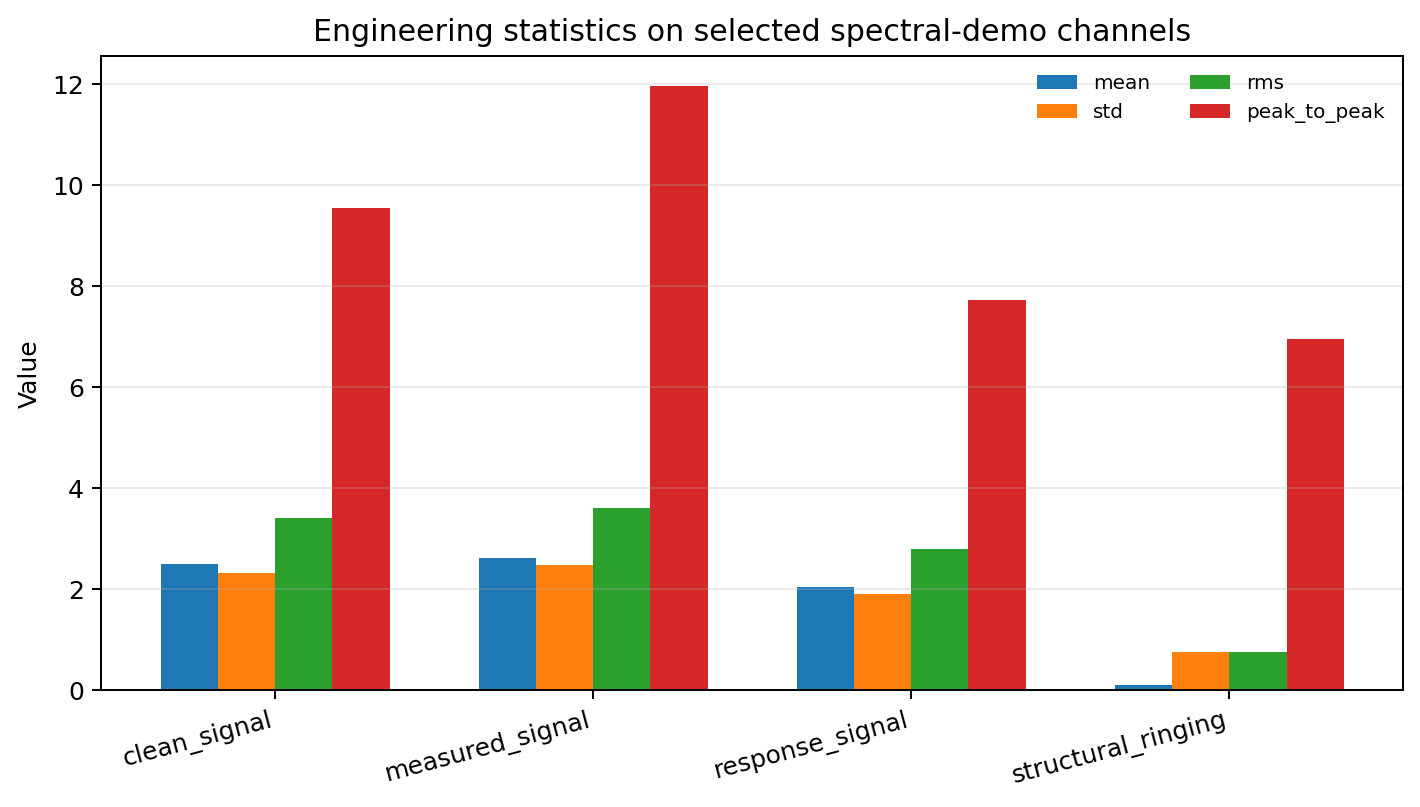
\includegraphics[width=0.92\linewidth]{statistics_metric_comparison.png}
    \caption{Selected engineering statistics for reproducible channels from the built-in spectral demo. The noisy and ringing-affected channels show larger spread than the clean reference signal.}
\end{figure}

\section{Correlation Matrix}

The current correlation view uses Pearson correlation on numeric columns. For signals $x$ and $y$,

\[
r_{xy} = \frac{\sum_{i=1}^{n}(x_i - \mu_x)(y_i - \mu_y)}{\sqrt{\sum_{i=1}^{n}(x_i - \mu_x)^2} \sqrt{\sum_{i=1}^{n}(y_i - \mu_y)^2}}.
\]

This produces values in $[-1, 1]$:

\begin{itemize}
    \item $r \approx 1$: strong positive linear relationship,
    \item $r \approx -1$: strong negative linear relationship,
    \item $r \approx 0$: weak linear relationship.
\end{itemize}

\begin{figure}[ht]
    \centering
    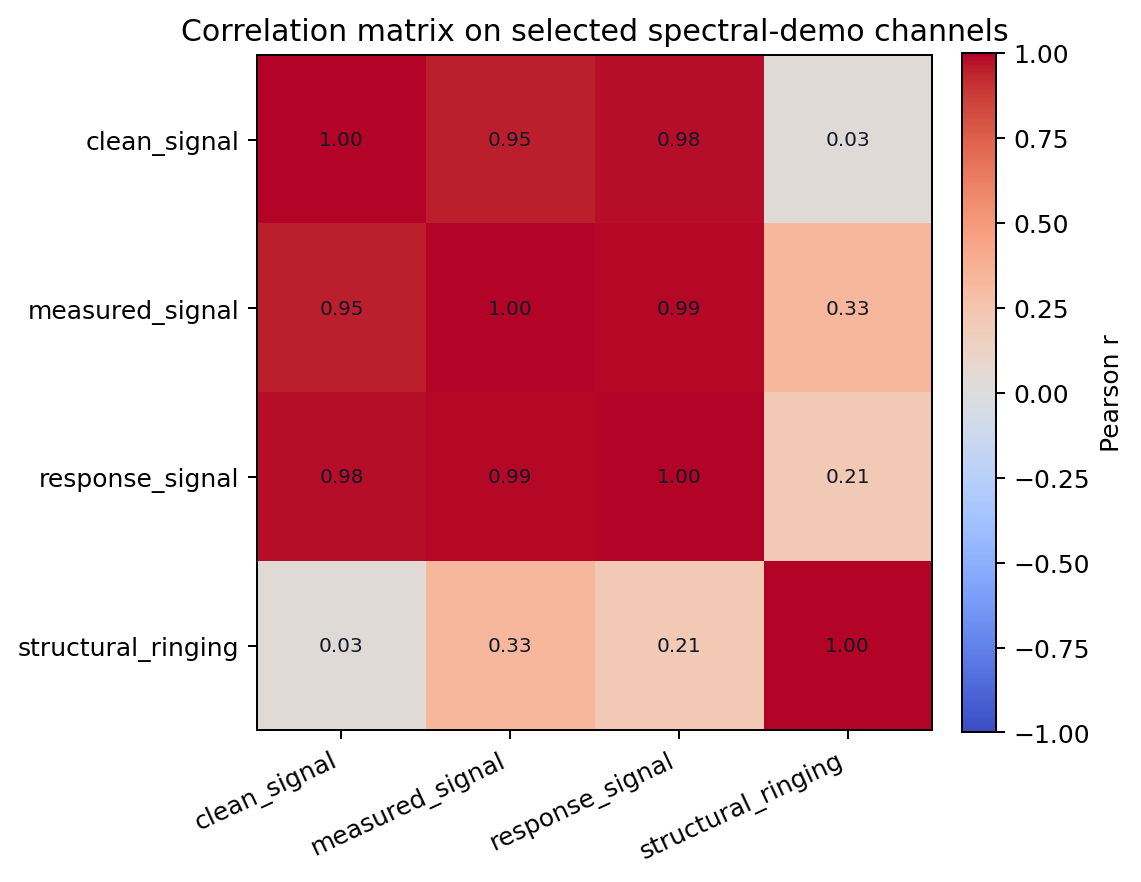
\includegraphics[width=0.82\linewidth]{correlation_heatmap_example.png}
    \caption{Correlation matrix for selected channels from the built-in spectral demo. The measured and response channels stay strongly related to the clean signal, while the ringing channel is more specialized.}
\end{figure}

\section{What the Demo Shows}

The spectral demo is useful because it combines one clean reference signal, one noisier measured signal, one related response signal, and one isolated ringing component. That gives the statistics and correlation views enough structure to show meaningful differences while remaining deterministic.

\section{Practical Interpretation Limits}

\begin{itemize}
    \item These statistics summarize the current working dataframe only. If the user filters or derives new columns, the reported values change accordingly.
    \item Pearson correlation measures linear association, not causality.
    \item Strong correlation can come from shared trends or shared periodic content, not necessarily from a direct physical mechanism.
    \item RMS and standard deviation are related but not identical, especially when the signal has a nonzero mean.
\end{itemize}

\section{Conclusion}

EvalData's statistics and correlation views are mathematically standard but practically important. They provide a compact numeric description of the current working dataframe and make it easier to verify whether transformations changed the signal in the way the user expected.

\begin{thebibliography}{9}

\bibitem{bendat2010}
J.~S.~Bendat and A.~G.~Piersol,
\emph{Random Data: Analysis and Measurement Procedures}, 4th~ed.
Hoboken, NJ: Wiley, 2010.

\bibitem{papoulis2002}
A.~Papoulis and S.~U.~Pillai,
\emph{Probability, Random Variables, and Stochastic Processes}, 4th~ed.
New York, NY: McGraw-Hill, 2002.

\end{thebibliography}

\end{document}